%==================================================================================================
% LaTeX paper template - use as a starting point for structuring a research paper.
%
% Written by Colin Perkins (https://csperkins.org/)
% 2002-2018
%
% To the extent possible under law, the author(s) have dedicated all copyright and
% related and neighbouring rights to this software to the public domain worldwide.
% This template is distributed without any warranty.
%
% You should have received a copy of the CC0 Public Domain Dedication along with
% this software. If not, see <http://creativecommons.org/publicdomain/zero/1.0/>.
%
% NOTE: The above Public Domain Dedication applies only to the LaTeX paper
% template distributed from https://github.com/csperkins/project-template
% in the file papers/example.tex. Unless explicitly stated, modifications 
% or additions to that template are copyright by their respective authors.
%==================================================================================================

%==================================================================================================
% General advice on technical writing:
%  - George Gopen and Judith Swan, "The Science of Scientific Writing",
%    American Scientist, Nov/Dec 1990. 
%    http://www.americanscientist.org/issues/num2/the-science-of-scientific-writing/1
%  - Stephen Pinker, "The Sense of Style: The Thinking Person's Guide to
%    Writing in the 21st Century", Penguin, Sept 2014. ISBN 0525427929.
%
% The paper writing advice in the comments is derived from talks and articles
% by Simon Peyton-Jones, Jim Kurose, Henning Schulzrinne, and Jim Bednar: 
%  - http://research.microsoft.com/~simonpj/papers/giving-a-talk/giving-a-talk.htm
%  - http://research.microsoft.com/~simonpj/papers/giving-a-talk/writing-a-paper-slides.pdf
%  - http://gaia.cs.umass.edu/kurose/talks/top_10_tips_for_writing_a_paper.ppt
%  - http://www-net.cs.umass.edu/kurose/writing/intro-style.html
%  - http://www.cs.columbia.edu/~hgs/etc/writing-style.html
%  - http://homepages.inf.ed.ac.uk/jbednar/writingtips.html
%  - http://www.gabbay.org.uk/blog/paper-writing.html
%  - http://homes.cs.washington.edu/~mernst/advice/write-technical-paper.html
%  - http://dx.doi.org/10.1371/journal.pcbi.1005619
%
% LaTeX usage notes:
%  - http://www.read.seas.harvard.edu/~kohler/latex.html
%
%==================================================================================================

%==================================================================================================
% The \documentclass{} macro specifies the overall style. For computer
% networking papers, common options are:
%
%   \documentclass[twocolumn,a4paper]{article}  % Base LaTeX style
%   \documentclass[conference]{IEEEtran}        % IEEE Conference
%   \documentclass[10pt,sigconf]{acmart}        % ACM SIGCOMM conference
%
% The IEEE and ACM templates are included in the lib/tex/inputs directory,
% but check for updates and use the version specified by the conference or
% journal to which you're submitting.

\documentclass[10pt,sigconf,anonymous]{acmart}
\synctex=1
\graphicspath{{figures/}{doc/paper/}}

% The following packages are recommended, and should be available in most
% standard LaTeX installations (or from https://www.ctan.org/). Note that 
% the order in which packages are loaded is significant.

% Basic extensions recommended for all LaTeX documents:
%   nag        Warn about common problems with LaTeX files
%   inputenc   Specify the character set used in .tex files
%   babel      Language-specific typography and hyphenation
%   microtype  Improved typography when generating PDF files

\usepackage[l2tabu,orthodox]{nag}
\usepackage[utf8x]{inputenc}
\usepackage[british]{babel}
\usepackage{ifpdf}
\usepackage{longtable}
\ifpdf
  \usepackage{microtype}
\fi

% The AMS mathematics library greatly extends and improves mathematics
% support in LaTeX (see http://ctan.org/pkg/amsmath for details). When
%  preparing multi-line numbered equations, be sure to use:
%
%   \begin{align}
%     ...
%   \end{align} 
%
% rather than:
%
%   \begin{eqnarray}
%     ...
%   \end{eqnarray}.  
%
% when this package is loaded, to ensure they formatting is consistent
% (see https://tug.org/pracjourn/2006-4/madsen/madsen.pdf for details).

\usepackage{amsmath}
\usepackage[all]{onlyamsmath}

% Use Times, Helvetica, and Courier fonts, rather than Computer Modern:

\makeatletter
\@ifclassloaded{acmart}{
  % The ACM article style sets the fonts internally
}{
  \usepackage{newtxtext}
  \usepackage{newtxmath}
}
\makeatother

% Add support for sub-figures within a figure, as follows:
%
%   \begin{figure}
%     \centering
%     \subfloat[caption for 1st subfloat]{
%       \includegraphics{...}
%       \label{...}
%     }
%     \\
%     \subfloat[caption for 2nd subfloat]{
%       \includegraphics{...}
%       \label{...}
%     }
%     \caption{caption for entire figure}
%     \label{...}
%   \end{figure*}
%
% The subfig package obsoletes the older subfigure package, and is itself
% deprecated in favour of the subcaption package. However, as of April 2015
% subcaption doesn't work with ACM or IEEE style files (this is also the
% reason for the [caption=false] option).

\usepackage[caption=false]{subfig}

% Improve formatting of tables. To produce nice looking tables:
%
%   - avoid vertical lines;
%   - avoid double horizontal lines;
%   - use horizontal lines above and below the table, and to separate the
%     header from the body of the table, but not elsewhere; and
%   - if in doubt, align columns to the left (columns of numbers should
%     align to the decimal point)
%
% This translates to a tabular environment that looks something like the
% following:
%
%   \begin{tabular}{lll}
%     \toprule
%        Header1 & Header2 & Header3 \\
%     \midrule
%        Line1   & ...     & ...     \\
%        Line2   & ...     & ...     \\
%        Line3   & ...     & ...     \\
%        Line4   & ...     & ...     \\
%     \bottomrule
%   \end{tabular}

\usepackage{booktabs}

% Improve formatting for quote marks in verbatim mode:
\usepackage{upquote}

% Improve support for graphics:
\usepackage{graphicx}

% Add support for URLs using \url{...}. This formats the URL in typewriter
% font, and makes it a hyperlink if the hyperref package is also loaded.
\usepackage{url}

% Add support for drawing packet headers. For instructions, see
% http://ctan.org/tex-archive/macros/latex/contrib/bytefield
\usepackage{bytefield}

% Add support for typesetting program source code. You can either include
% code in-line:
%
%   \begin{lstlisting}[language=Python]
%   Source code goes here
%   \end{lstlisting}
%
% or include a source file:
%
%  \lstinputlisting[language=Python]{source_filename.py}
%
% This package is highly customisable and supports a range of languages.
% See package documentation at https://ctan.org/pkg/listings for details.
\usepackage{listings}

% Generated PDF files can include hyperlinks for URLs and cross-references
% using the hyperref package. This package, however, can interact poorly
% with others. Known issues include:
%
%  - Papers typeset without page numbers gives warnings of the form:
%      "pdfTeX warning (ext4): destination with the same identifier 
%      (name{page.}) has been already used, duplicate ignored".
%    since hyperref tries to refer to the page number.
%  - The algorithmic package uses the same line-numbering scheme for each
%    algorithm, and can cause duplicate identifier warnings if you have
%    several algorithms with line numbers (this may have been fixed with 
%    recent versions of algorithmic...).
%  - If using the algorithm package with hyperref, you need to load packages
%    in the following order (see README in hyperref documentation):
%      \usepackage{float}
%      \usepackage{hyperref}
%      \usepackage{algorithm}
% For these reasons, hyperref is best to avoid for most papers, however if
% needed, uncomment the following two lines:
%  \usepackage{float}
%  \usepackage{hyperref}

% The algorithm package defines the algorithm environment. This is used in
% the same way as the figure and table environments, to include algorithms
% in a paper. The algpseudocode package provides the ability to typeset the
% algorithms: http://ctan.org/tex-archive/macros/latex/contrib/algorithmicx
\usepackage{algorithm}
\usepackage{algpseudocode}
\usepackage{color}


% By default, LaTeX adds extra space after punctuation. The \frenchspacing
% command disables this. This creates tighter looking, more even, text and
% avoids inconsistencies if you forget to use '\ ' to suppress the spacing
% after in-sentence punctuation.
\frenchspacing

% Prevent hyphenation of all upper case words:
%\uchyph=0

% The ACM style needs \maketitle after the abstract, but the other styles
% want it before; these macros hide the difference and are used below:
\makeatletter
\@ifclassloaded{acmart}{
  \newcommand{\maketitleSTD}{}
  \newcommand{\maketitleACM}{\maketitle}
}{
  \newcommand{\maketitleSTD}{\maketitle}
  \newcommand{\maketitleACM}{}
}
\makeatother

% Define a simple \todo{...} macro:
\newcommand{\todo}[1]{\textbf{\textcolor{red}{To do: #1}}}

\newcommand{\idea}[1]{{\textcolor{blue}{#1}}}

%==================================================================================================
\begin{document}
% Specify the title of the document:

\title{Does TCP's New Congestion Window Validation Improve HTTP Adaptive Streaming Performance?}

% Specify the authors of the document. Unfortunately, there's no consistent
% way to do this that works across the different document classes. 
%
% If using \documentclass{article}:
%
%   \author{
%      A. N. Other\\University of Glasgow
%   \and
%      Colin Perkins\\University of Glasgow
%   }
%
% If using \documentclass{IEEEtran}:
%
%   \author{
%     \IEEEauthorblockN{A. N. Other}
%     \IEEEauthorblockA{University of Glasgow}
%   \and
%     \IEEEauthorblockN{Colin Perkins}
%     \IEEEauthorblockA{University of Glasgow}
%   }
%
% If using \documentclass{acmart} add a block like the following per author:
%
%   \author{Colin Perkins}
%   \orcid{0000-0002-3404-8964}
%   \affiliation{
%     \institution{University of Glasgow}
%     \streetaddress{School of Computing Science}
%     \city{Glasgow}
%     \postcode{G12 8QQ}
%     \country{UK}
%   }
%   \email{csp@csperkins.org}
%
% If you don't have an ORCID identifier, sign up for one at https://orcid.org

\author{Mihail Yanev}
    %\orcid{0000-0002-3404-8964}
    \affiliation{
      \institution{University of Glasgow}
      \streetaddress{School of Computing Science}
      \city{Glasgow}
      \postcode{G12 8QQ}
      \country{UK}
    }
    \email{m.yanev.1@research.gla.ac.uk}


\author{Stephen McQuistin}
    % \orcid{0000-0002-3404-8964}
    \affiliation{
    \institution{University of Glasgow}
    \streetaddress{School of Computing Science}
    \city{Glasgow}
    \postcode{G12 8QQ}
    \country{UK}
    }
    \email{}

\author{Colin Perkins}
  \orcid{0000-0002-3404-8964}
  \affiliation{
    \institution{University of Glasgow}
    \streetaddress{School of Computing Science}
    \city{Glasgow}
    \postcode{G12 8QQ}
    \country{UK}
  }
  \email{csp@csperkins.org}



% Specify metadata about the paper. Again, what is required depends on the
% document class. If using \documentclass{acmart}, specify the following:
%
%   \acmYear{2018}
%   \copyrightyear{2018}
%   \setcopyright{acmcopyright}
%   \acmConference{CoNEXT '18}{December 4--7, 2018}{Heraklion/Crete, Greece}
%   \acmPrice{15.00}
%   \acmDOI{10.1145/3284850.3284856}
%   \acmISBN{978-1-4503-6082-1/18/12}
%
% The complete metadata is likely only available when preparing the final,
% camera ready, version of the paper.

\acmYear{2021}
\copyrightyear{2021}
\setcopyright{acmcopyright}
\acmConference{NOSSDAV '22}
% {December 4--7, 2018}{Heraklion/Crete, Greece}
\acmPrice{15.00}
% \acmDOI{10.1145/3284850.3284856}
% \acmISBN{978-1-4503-6082-1/18/12}

%==================================================================================================
\maketitleSTD
\begin{abstract}
  % Four sentences:
  %  - State the problem
  %  - Say why it's an interesting problem
  %  - Say what your solution achieves
  %  - Say what follows from your solution

HTTP adaptive streaming video flows exhibit on-off behaviour, with frequent idle periods, which can interact poorly with TCP's congestion control algorithms. New Congestion Window Validation (New CWV) modifies TCP to allow senders to restart more quickly after certain idle periods. While previous work has shown that New CWV can improve \emph{transport} performance for streaming video, it remains to demonstrate that this translates to improved \emph{application} level performance, in terms of playback stability. In this paper, we show that enabling New CWV can reduce video re-buffering events by up to 4\%, and limit representation switches by 12\%, without any changes to existing rate adaptation algorithms.

\end{abstract}
\maketitleACM


\section{Introduction}
\label{sec:introduction}

% A good paper introduction is fairly formulaic. If you follow a simple set
% of rules, you can write a very good introduction. The following outline can
% be varied. For example, you can use two paragraphs instead of one, or you
% can place more emphasis on one aspect of the intro than another. But in all
% cases, all of the points below need to be covered in an introduction, and
% in most papers, you don't need to cover anything more in an introduction.
%

Video streaming over HTTP is commonplace, and comprises the majority of Internet traffic~\cite{Sandvine-2019-global-internet-report}. Performance of HTTP adaptive streaming is generally good, and gives a high-quality user experience~\todo{\cite{..}}.
  
There remain, however, scenarios where HTTP adaptive streaming performs poorly~\cite{Spiteri-2016-BOLA,Kua-2017-a-survey-rate-adaptation-dash}. In particular, it has been observed that the interaction between the on-off traffic patterns generated by chunked streaming applications and TCP's congestion control algorithms reduces the performance of throughput-based rate adaptation schemes~\cite{Akhshabi-2012-http-adaptive-players-compete,Stohr-2017-where-are-the-sweet-spots-maci}. In some cases, this is due to TCP's Congestion Window Validation (CWV)~\cite{rfc2861-2000-padhye-congestion-window-validation} algorithm, which, while preventing TCP clients from sending using stale knowledge of the network, has been shown to negatively impact the throughput of rate-limited applications~\cite{Nazir-2014-performance-evaluation-congestion-window-validation-dash-newcwv}, including HTTP adaptive streaming. New Congestion Window Validation (New CWV)~\cite{rfc7661-2015-fairhurst-new-cwnd-validation} has been proposed to address this. Prior work~\cite{Nazir-2014-performance-evaluation-congestion-window-validation-dash-newcwv} has demonstrated that New CWV has the desired \emph{transport} layer impact, but it remains to show that this translates to improved quality of experience (QoE) performance at the \emph{application} layer. This is not guaranteed, given the complexity that exists at both layers, and that results from their interaction. For example, large discrepancies between the video's bandwidth requirements and the available link capacity, or the requirement for stable, long-lived connections in modern streaming video players (e.g., dash.js~\cite{online-dashjs}), can influence rate adaptation~\cite{Spiteri-2019-from-theory-to-practice-sabre}.

% Paragraph 1: Motivation. At a high level, what is the problem area you
% are working in and why is it important? It is important to set the larger
% context here. Why is the problem of interest and importance to the larger
% community?

% Video playback stability is one of the key components contributing to user experience. Adaptive algorithms residing at the client are responsible for delivering high user experience. Some current state-of-the-art solutions use network throughput as a bitrate selection heuristic.

% Paragraph 2: What is the specific problem considered in this paper? This
% paragraph narrows down the topic area of the paper. In the first
% paragraph you have established general context and importance. Here you
% establish specific context and background.

% The adaptive algorithms face the difficult task of delivering video while picking its ``best'' representations at any given point in time. This is since these algorithms need to simultaneously fulfil multiple criteria including: high stability, high quality, and low video stalls. These criteria can often conflict one another. For example, an algorithm always picking the lowest available representation will achieve low video stall time and high stability (since representations will not fluctuate), however, it will also display lower video quality, whereas perhaps higher one was possible. In a dynamic network, achieving a high index on one of these criterion also comes at the cost of observing a lower index in another. Modern adaptive algorithms try to balance that trade-off. They use either the pre-buffered capacity at the client or the immediate network state as a heuristic to aid them in the decision process. The former algorithms are known as buffer and the latter as throughput based. 


% One way to influence the client's throughput calculations is to change the transport. Video over HTTP has to transfer many video chunks over the same connection. The time when between each such transfers, when no information is exchanged, is known as an ``idle period''. RFC 5861 recommends that during such periods TCP should adjust its congestion window back to its initial window value and re-enter slow start \cite{rfc5681-congeston-control}. New Congestion Window Validation \cite{rfc7661-2015-fairhurst-new-cwnd-validation} proposes a way for the congestion window value to remain unchanged during idle periods and connections using it do not need to re-enter slow start. These two approaches have different impact on the client's throughput calculations.


% However, different client throughput estimations does not necessarily mean improved video QoE. Video QoE is a complex variable that is a combination of different application metrics, e.g., average bitrate, average bitrate oscillation, and rebuffer ratio. As discussed earlier, improving one could come at the cost of worsening others. Therefore, the implications of a transport change are unclear with respect to the video's QoE or smoothness.


% Paragraph 3: "In this paper, we show that...". This is the key paragraph
% in the introduction - you summarize, in one paragraph, what are the main
% contributions of your paper, given the context established in paragraphs
% 1 and 2. What's the general approach taken? Why are the specific results
% significant? The story is not what you did, but rather:
%  - what you show, new ideas, new insights
%  - why interesting, important?
% State your contributions: these drive the entire paper.  Contributions
% should be refutable claims, not vague generic statements.

In this paper, we investigate whether enabling New CWV improves video playback stability, and more generally, improves video QoE. To test our hypothesis, we compare two video streams using TCP New Reno, one with CWV and with New CWV. We collect standard video performance metrics, including bit-rate oscillation, and stall time, to measure stability and QoE. Further, to quantify the impact of New CWV with respect to the inferred network state at the client, we also record the immediate and smoothened client's current link capacity estimations for each delivered video chunk.% We carry our experiments using TCP New Reno, as previous study found that it is widely used for video delivery \cite{Mishra-2019-the-great-internet-tcp-congestion-control-census} and because New CWV is agnostic to the used congestion control algorithm.
In specific, we make the following contributions: We provide a New CWV implementation for the most recent Linux Kernel series (5.4) \textit{Link to appear after anonymization is lifted}, created an environment that can be used for video testing, and carry out a study on New CWV's impact on the application layer concluding that New CWV improves video stability. 

% Paragraph 4: What are the differences between your work, and what others
% have done? Keep this at a high level, as you can refer to future sections
% where specific details and differences will be given, but it is important
% for the reader to know what is new about this work compared to other work
% in the area.

To the best of our knowledge, this is the first paper that studies New CWV's application layer impact. Nazir et al. \cite{Nazir-2014-performance-evaluation-congestion-window-validation-dash-newcwv} demonstrated New CWV's effect on the transport layer, and we validate their results. There has been a large amount of work that has proposed new application layer rate adaptation algorithms~\cite{Mok-2012-qdash,Huang-2015-A-buffer-based-approach-to-rate-adaptation-bba, Yin-2015-a-control-theoritic-approach}. In contrast, we only change the transport algorithm and leave the application as is, studying the transport's impact on the application. Improving performance via transport layer modifications allows for simpler rate adaptation algorithms at the application layer. %Another proposal considers replacing the transport protocol from TCP to QUIC \cite{Bhat-2017-not-so-quic} but find that only doing this brings little to no benefit. 

% Paragraph 5: "We structure the remainder of this paper as follows." Give
% the reader a road-map for the rest of the paper. Try to avoid redundant
% phrasing, "In Section 2, In section 3, ..., In Section 4, ... ", etc.

We structure the remainder of this paper as follows. In Section~\ref{sec:background}, we introduce TCP congestion window validation and motivate our work, Section~\ref{sec:evaluation} describes our experimental setup and obtained results. Section~\ref{sec:related} describes related work, and Section~\ref{sec:conclusion} concludes.

%==================================================================================================
\section{Congestion Window Validation}
\label{sec:background}

\begin{figure}
  \centering
    \subfloat[New CWV]{
      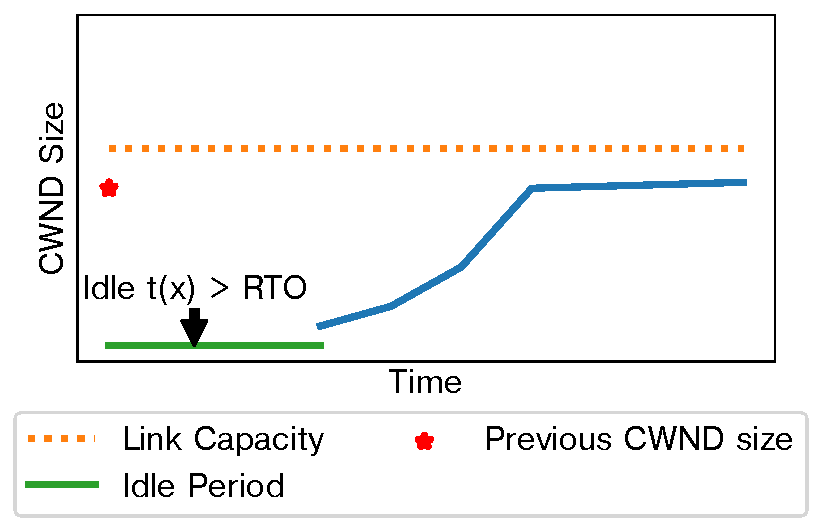
\includegraphics[width=.23\textwidth,]{figures/new_cwv.pdf}
      \label{fig:newcwv}
    }
    \subfloat[CWV]{
      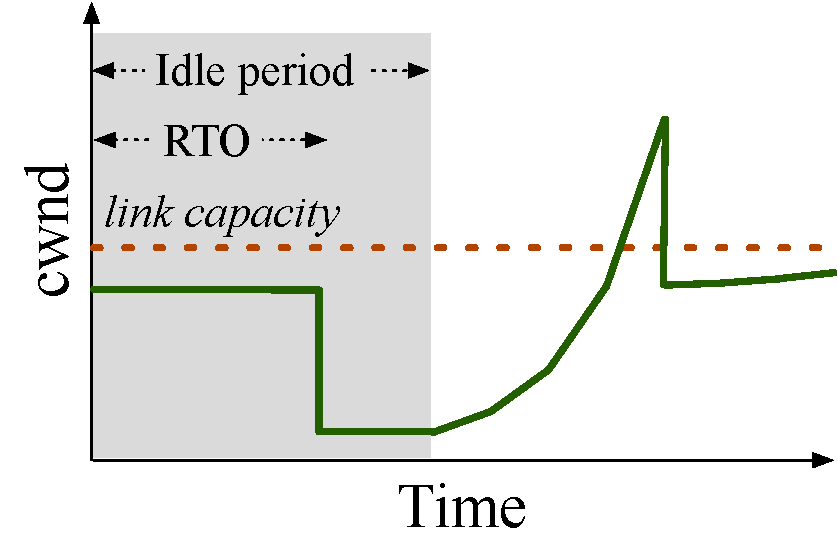
\includegraphics[width=.23\textwidth]{figures/cwv.pdf}
      \label{fig:cwv}
    }

    \caption{Illustration of CWND Growth After Idle}
    \label{fig:cwnd-growth-after-idle}
\end{figure}


In HTTP adaptive streaming, a server provides pre-encoded video chunks in different representations, each encoded at multiple bit rates, while the client, using a rate adaptation algorithm, determines the best representation to request at any given time. The goal of the client is to maximise QoE within the network's capacity. This is a challenge: different, often contradictory, QoE heuristics need be considered simultaneously~\cite{Seufert-2015-A-Survey-on-QoE-Dash}. 
% Furthermore, since HTTP streaming uses mainly TCP to transfer the chunks, the bit rate selection's algorithm complexity rises.

Throughput-based rate adaptation algorithms use an estimate of the current network conditions to determine the representation that should be requested. These algorithms require a stable and accurate estimate in order to perform well. However, the interaction between the on-off traffic pattern of streaming video and TCP congestion control algorithm, can lead to significant fluctuations in throughput, impacting the performance of throughput-based rate adaptation algorithms.

%Previous work has identified that the interaction between TCP and HTTP can lead to poor link utilisation and perceived quality of experience for HTTP adaptive connections \cite{Bae-2015-why-is-http-streaming-hard,Esteban-2012-Interactions-HTTP-TCP}. One impeding performance aspect of the interaction between the two layers is related to the On-Off nature of the video traffic.

During the off periods in the video transmission, the TCP congestion controller's knowledge of the network capacity becomes stale. To avoid sending with a possibly unrepresentative window, the Congestion Window Validation~\cite{rfc2861-2000-padhye-congestion-window-validation} algorithm resets the TCP congestion window (\texttt{cwnd}) to its initial value and forces the connection to re-enter slow-start after an idle period. This has become standard practice~\cite{rfc5681-congeston-control}, and is enabled by default in the latest stable Linux kernel (5.4).

While this approach has been employed and works for bulk, network-limited applications. It is unsuitable for rate-limited applications, including HTTP adaptive streaming~\cite{Esteban-2012-Interactions-HTTP-TCP}. To address this, New Congestion Window Validation~\cite{rfc7661-2015-fairhurst-new-cwnd-validation} has been proposed. One of New CWV's modification is that rather than relying on loss to re-discover an appropriate CWND value after an idle period, New CWV preserves the CWND before the idle period as its slow-start threshold (\emph{ssthresh}), i.e., it uses that value to later exit the slow-start phase (Figure~\ref{fig:cwnd-growth-after-idle}).

\begin{figure}[t!]
  \centering
    \subfloat[New CWV]{
      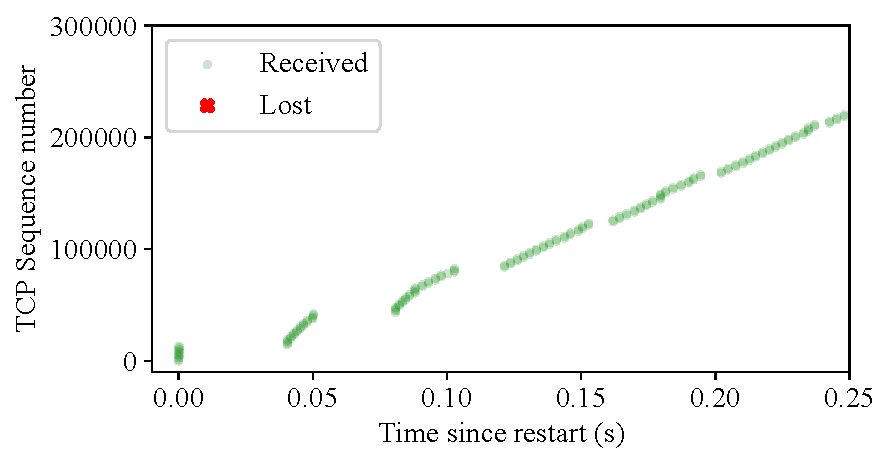
\includegraphics[width=.45\textwidth, keepaspectratio]{figures/lost_packets_newcwv.pdf}
      \label{fig:transmission-after-idle-newcwv}
    }
    \\
    \subfloat[CWV]{
      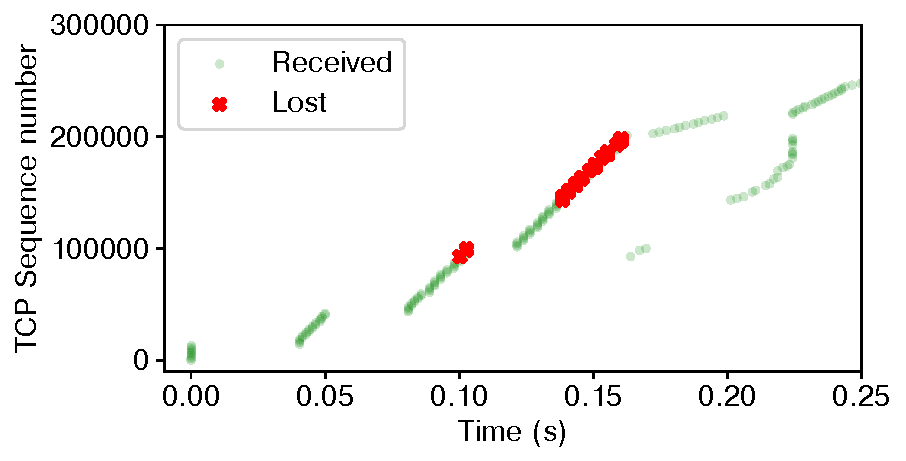
\includegraphics[width=.45\textwidth, keepaspectratio]{figures/lost_packets_vreno.pdf}
      \label{fig:transmission-after-idle-reno}
    }

    \caption{Resumption after an idle period}
    \label{fig:transmission-after-idle}
\end{figure}

The impact of New CWV is shown on Figure~\ref{fig:transmission-after-idle}. In it, the connection using New CWV uses the previously set \emph{ssthresh} value and leaves slow-start early. This results in New CWV connections not experiencing any packet loss (Figure~\ref{fig:transmission-after-idle-newcwv}), after reaching their set \emph{ssthresh} value in the third burst. In contrast, if the same connection used CWV, the senders would not have preserved the \emph{ssthresh} value that way and would rely on loss to exit slow start: forth burst and end of third (Figure~\ref{fig:transmission-after-idle-reno}). Overall, New CWV results in fewer lost packets, and returns to its previous sending rate without overshoot after loss, giving more predictable transmission.

New CWV has been shown to improve the \emph{transport} layer performance of rate-limited applications when compared with CWV~\cite{Nazir-2014-performance-evaluation-congestion-window-validation-dash-newcwv}. It remains to show how this translates into \emph{application} layer performance, particularly since this is not guaranteed~\cite{Spiteri-2016-BOLA}. We hypothesise that New CWV will enable applications to obtain more consistent throughput estimates, and, in turn, improve the stability of throughput-based rate adaptation algorithms.

%==================================================================================================
\section{Evaluating New CWV for Video}
\label{sec:evaluation}

\begin{figure}
  \centering
  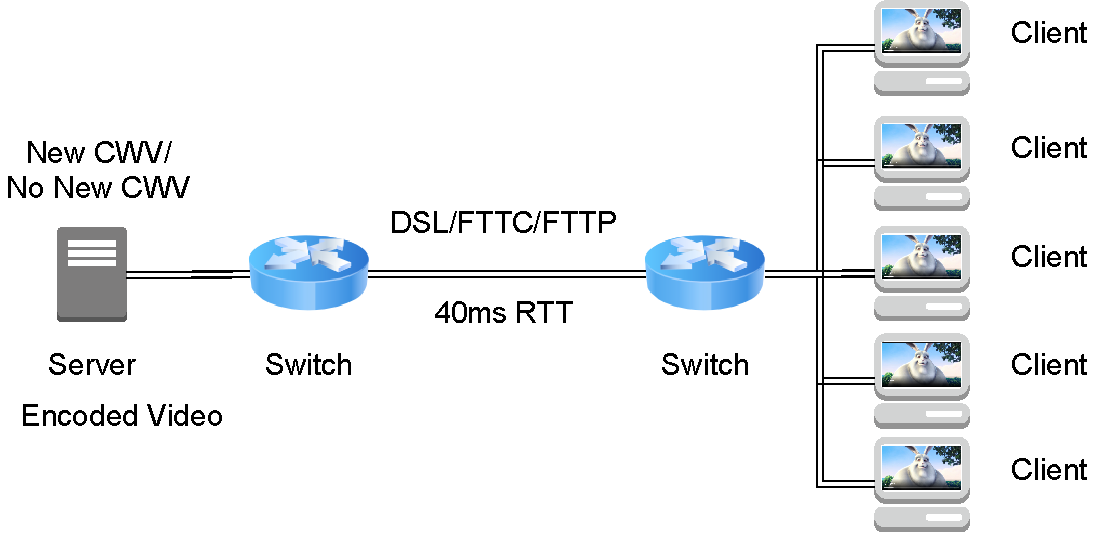
\includegraphics[width=.5\textwidth]{figures/setup.pdf}
  \caption{Experimental Setup}
  \label{fig:experimental-setup}
\end{figure}

We first describe our experimental setup (\S\ref{sec:experimental-setup}), and use this to look at the impact on the transport layer, and measure the extent to which streaming applications using New CWV obtain more consistent throughput estimates (\S\ref{sec:transport-impact}). We then investigate how this transport behaviour impacts the application layer, and, more specifically, video QoE (\S\ref{sec:QoE-impact}). Finally,  we summarise our findings (\S\ref{sec:summary}).

%--------------------------------------------------------------------------------------------------
\subsection{Experimental Setup}
\label{sec:experimental-setup}



% Overview
Our evaluation testbed consists of an emulated network in Mininet, running on Ubuntu 20.04, as shown in Figure \ref{fig:experimental-setup}. Both the server and its clients use TCP New Reno, which is widely used for video delivery~\cite{Mishra-2019-the-great-internet-tcp-congestion-control-census}. In addition, both are running a modified Linux Kernel (5.4.0). The modifications include a version of New CWV ported to that kernel, alongside RFC 3339~\cite{rfc3339-precise-timestamps}-compliant timestamps, to enable better event tracking, and more verbose \texttt{cwnd} event tracking. \texttt{tcpdump} is used at all endpoints to enable network activity to be reconstructed.

% Server
The server uses \texttt{nginx} (version 1.18), with HTTP/2 delivery enabled. The server provides three representations of Big Buck Bunny~\cite{online-bbb}, encoded at 480p (requiring bandwidth of 0.44Mbps), 720p (2.64Mbps), and 1080p (4.82Mbps). Each representation is provided in chunks that are 3 seconds in duration.

 %  Client
Each client uses Firefox (version 91) with the dash.js (version 4.0.0) player. While the current state-of-the-art rate adaptation algorithm is DYNAMIC~\cite{Spiteri-2019-from-theory-to-practice-sabre}, we opt to use the throughput algorithm for our experiments. DYNAMIC combines the throughput algorithm with an enhanced version of the BOLA algorithm~\cite{Spiteri-2016-BOLA}. By using the throughput algorithm, our evaluations focus on the impact that the transport layer has on throughput estimation at the application layer. Our findings are applicable to the DYNAMIC algorithm, especially in scenarios where the throughput algorithm operates (e.g., in low-latency, live streaming applications).

The network is configured a bottleneck RTT of 40ms, a reasonable value to emulate connections within the UK. The routers' queues are set equal to the bandwidth delay product. Three different bandwidth profiles are evaluated, representing DSLv2 (10Mbps), FTTC (50Mbps), and FTTP (145Mbps) links in the UK~\cite{online-ofcom-report} Below we show mostly the results for the DSLv2 and FTTC links as the number of clients and the video representation demands were always unable to saturate an FTTP link's capacity. However, as higher resolution video and other network-heavy operations such as virtual reality environments become more available we expect these issues to translate to the links with higher capacity (i.e. FTTP).

To evaluate the impact of congestion and competing flows, each simulation was run with multiple clients (1, 2, 3, and 5 clients) simultaneously requesting video. Finally, to reduce noise, we ran each combination of CWV or New CWV, number of clients, and link type, 10 times before reporting the average results. The dataset presented includes data accumulated from 240 simulations (\emph{2 algorithms $\times$ 3 link types $\times$ 4 client variations $\times$ 10 repetitions}). 

During each run we collect the client's bandwidth estimations. Additionally, to evaluate the video QoE impact we collect information to report the rebuffer ratio and the bitrate switch frequency distribution.

%--------------------------------------------------------------------------------------------------
\subsection{Impact on Transport Performance} 
\label{sec:transport-impact}

New CWV alters the CWND sizing behaviour, allowing it to recover faster, after an idle period in an active TCP connection. Therefore, we expect the client to report more stable values regarding the available link bandwidth. 

To evaluate our hypothesis, we collect two of the client's available bandwidth measurements. The first, we call ``smoothed'' is the estimate obtained by dividing the number of received bytes over the download time. The second, we call ``instantaneous'' is the estimate that gets fed to the throughput algorithm. This value is a function of the current immediate measurement, and additional factors including, historical measurement data, ``safety" or smoothening factors, etc. In short, the former is the available bandwidth measurement as seen by end-point, and the latter is the input value to the algorithm.

\begin{figure*}[t!]
  \centering
  \subfloat[DSL]{
    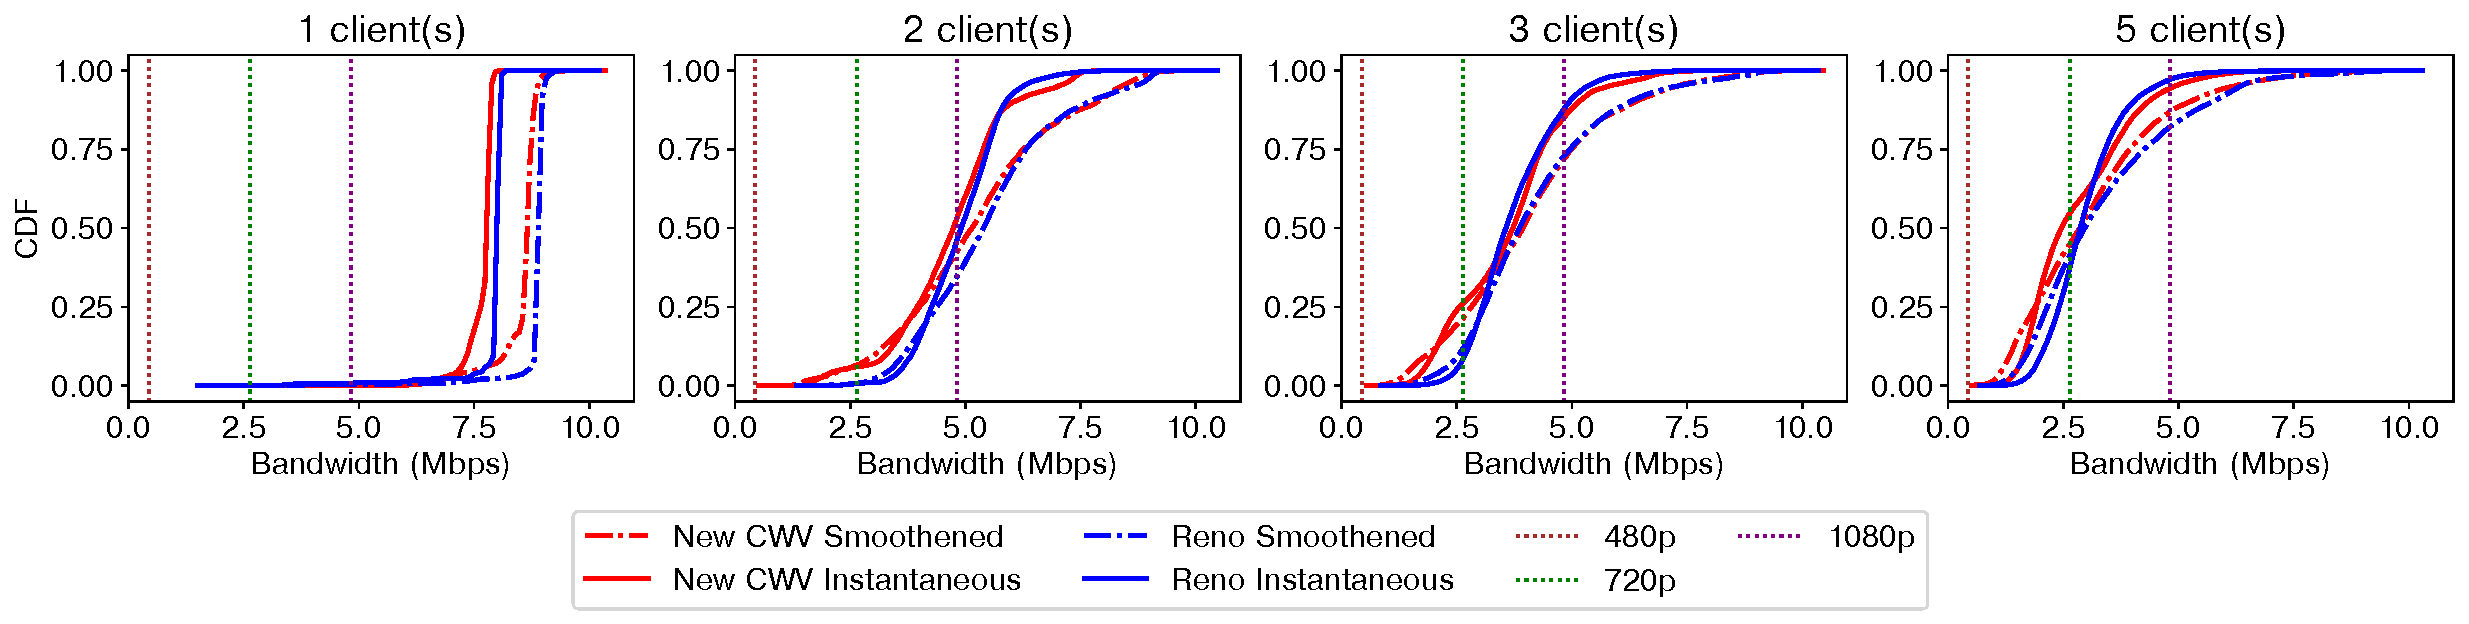
\includegraphics[width=\textwidth]{figures/Throughput_DSL.pdf}
    \label{fig:throughput-clients-DSL}
  }
  \\
  \subfloat[FTTC]{
    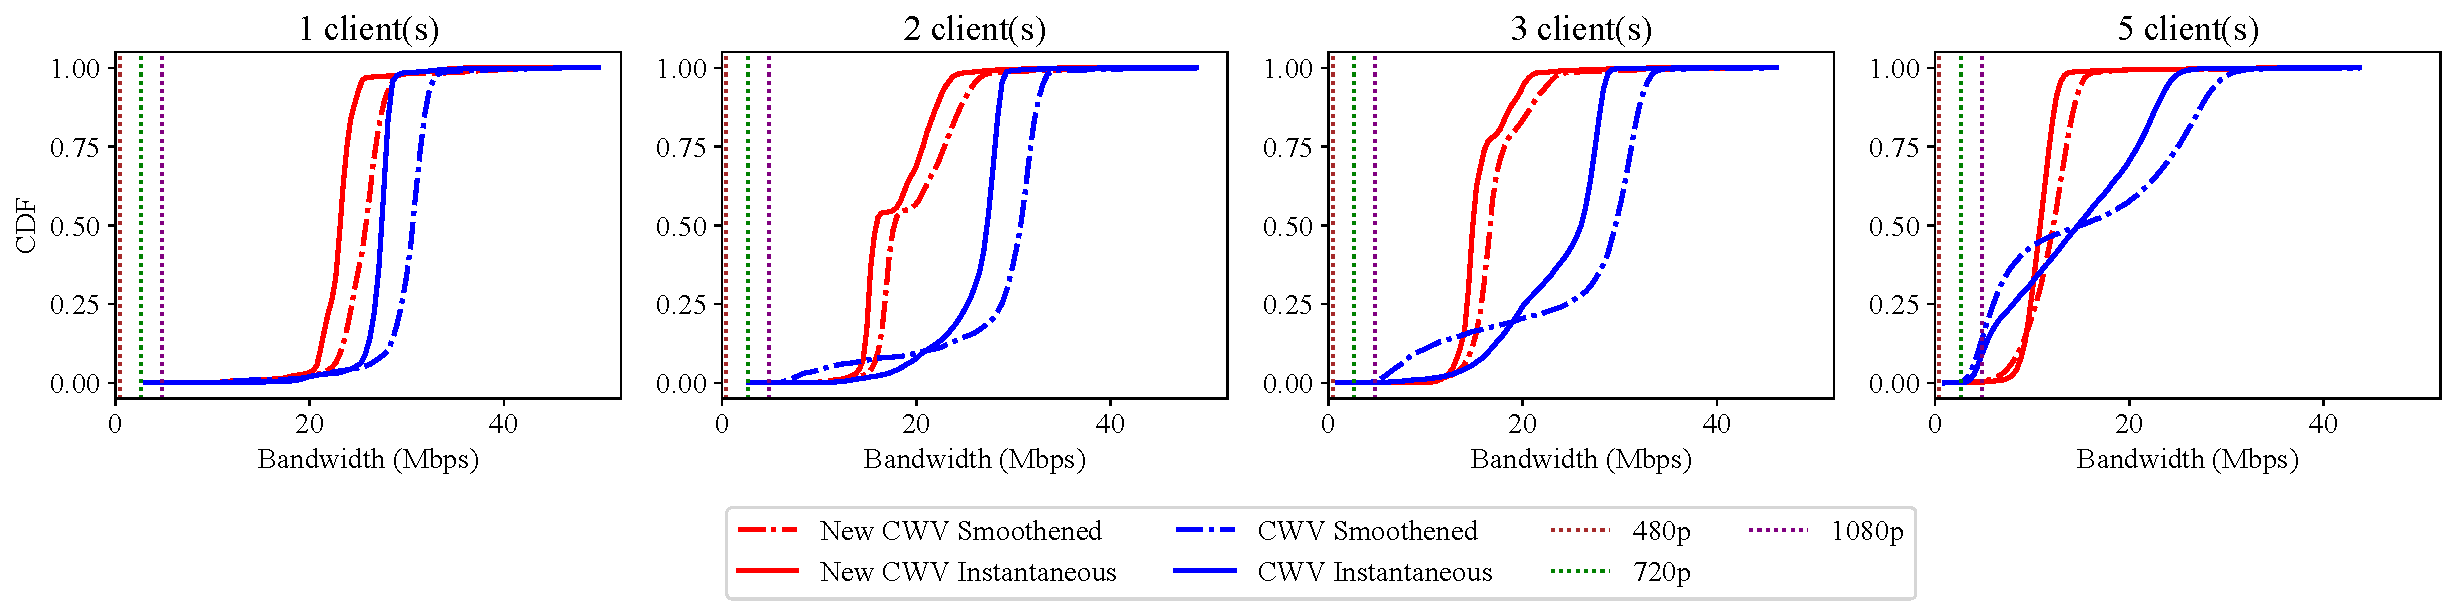
\includegraphics[width=\textwidth]{figures/Throughput_FTTC.pdf}
    \label{fig:throughput-clients-FTTC}
  }
  \caption{Dash.js Client Throughput measurements}
  \label{fig:throughput-clients}
\end{figure*}

Figure \ref{fig:throughput-clients} validates the behaviour when New CWV is enabled, as reported by \cite{Nazir-2014-performance-evaluation-congestion-window-validation-dash-newcwv}. This supports our initial hypothesis that the streaming clients measuring the available bandwidth will be able to obtain more consistent. This is consistent with the behaviour seen in Figure \ref{fig:transmission-after-idle}. Figure \ref{fig:throughput-clients} shows that the obtained measurements are more consistent. For example, in all FTTC scenarios (Figure \ref{fig:throughput-clients-FTTC}), New CWV has a steeper gradient. This means the available bandwidth values there were more consistent. This is because, since New CWV is able to leave its slow-start earlier, its CWND oscillates less, than that of CWV. It should also be noted that when using New CWV while the reported values are more consistent, they were also lower, compared to these achieved by CWV. This is since, CWV would always reach the maximum link capacity because of its longer slow-start phase. However, as we show later these higher values could lead the throughput algorithm into making bit-rate selection decisions that cannot be supported by the network layer.

\begin{figure}[t!]
  \centering
  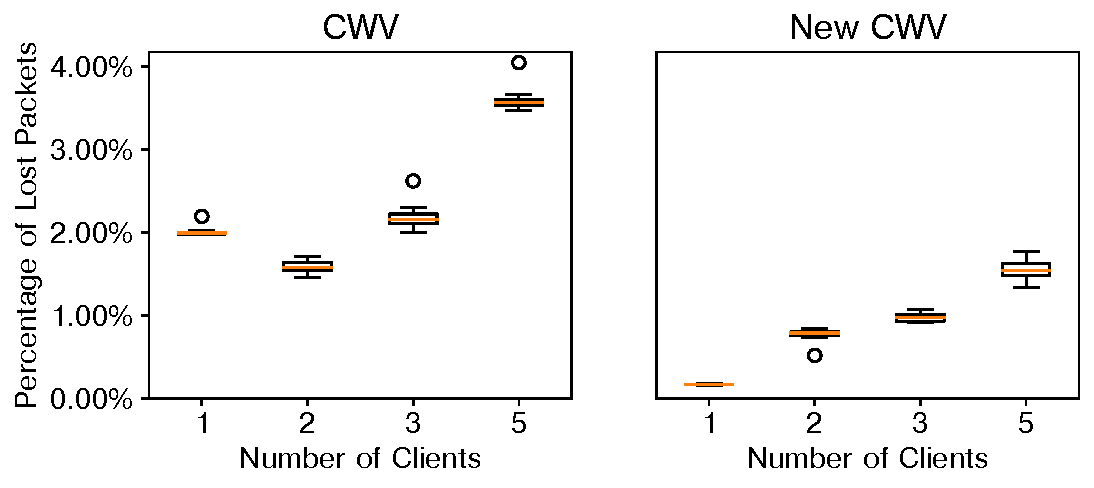
\includegraphics[width=.45\textwidth]{figures/lost_packets.pdf}
  \caption{Lost Packets DSL}
  \label{fig:lost-packets}
\end{figure}

Our packet loss results (Figure \ref{fig:lost-packets}) show that New CWV consistently achieves lower loss rates compared to standard CWV. We see that New CWV connections have as high as 2\% less overall lost packets in the 1 and 5 client scenarios. This is because, as explained in Section \ref{sec:background}, New CWV exits slow-start earlier, does not overshoot its window, and therefore is able to avoid the loss seen near the end of slow-start that CWV observes \ref{fig:transmission-after-idle}. \cite{Nazir-2014-performance-evaluation-congestion-window-validation-dash-newcwv} observed similar loss values both when New CWV is enabled and when it is not. We attribute that to the much larger RTT value they used.

% To evaluate this hypothesis, we collect two of the client's available bandwidth measurements. The first is the raw estimate obtained by dividing the number of received bytes by time taken to download them. The second estimation, used by the application level adaptation algorithm, is a function of the raw bandwidth estimate, already explained, and additional factors, including historical values. We refer to the former as the \emph{instantaneous} and the latter the \emph{smoothed} estimate.

% Figure~\ref{fig:throughput-clients} shows CDFs of the instantaneous and smoothed bandwidth estimates. Intuitively, steeper lines indicate more consistent estimates: that is, a greater proportion of the estimates fall within a tighter range of values. As shown in Figure~\ref{fig:throughput-clients}, New CWV tends to report bandwidth estimates that are more consistent. This validates both our initial hypothesis, and the results reported by Nazir et al.~\cite{Nazir-2014-performance-evaluation-congestion-window-validation-dash-newcwv}. We also find that New CWV produces bandwidth estimates that are lower overall. This is since when New CWV is enabled, connections will not hit the available capacity cap as fast. However, this pre-emptive mechanism allows for higher consistency on links where nearly all of the available bandwidth is used (FTTC scenarios in Figure \ref{fig:throughput-clients}). \todo{not sure what the last couple of sentences are trying to say}.


% However, our packet loss results (Figure \ref{fig:transmission-after-idle}) differ from those reported by Nazir et al.~\cite{Nazir-2014-performance-evaluation-congestion-window-validation-dash-newcwv}. They observed similar loss values with and without New CWV enabled, while we observe that when disabled, connections lose more packets (at a rate close to 1:10) compared to when enabled. Figure \ref{fig:transmission-after-idle} shows the transfer patterns for a single video chunk after an idle period. It can be seen that when New CWV is disabled the majority of the packets lost are near the end of the slow-start period, when the \texttt{cwnd} size allows for transferring data beyond the link's capacity \todo{words, backref to sec 2 diagram}. In contrast, since New CWV enters slow-start with an upper bound of its previous window value, New CWV is able to enter congestion avoidance faster without losing packets as a result of a large \texttt{cwnd} value. This explains the higher loss values that we have observed.

%--------------------------------------------------------------------------------------------------
\subsection{Impact on Video QoE}
\label{sec:QoE-impact}

\begin{figure*}
  \centering
  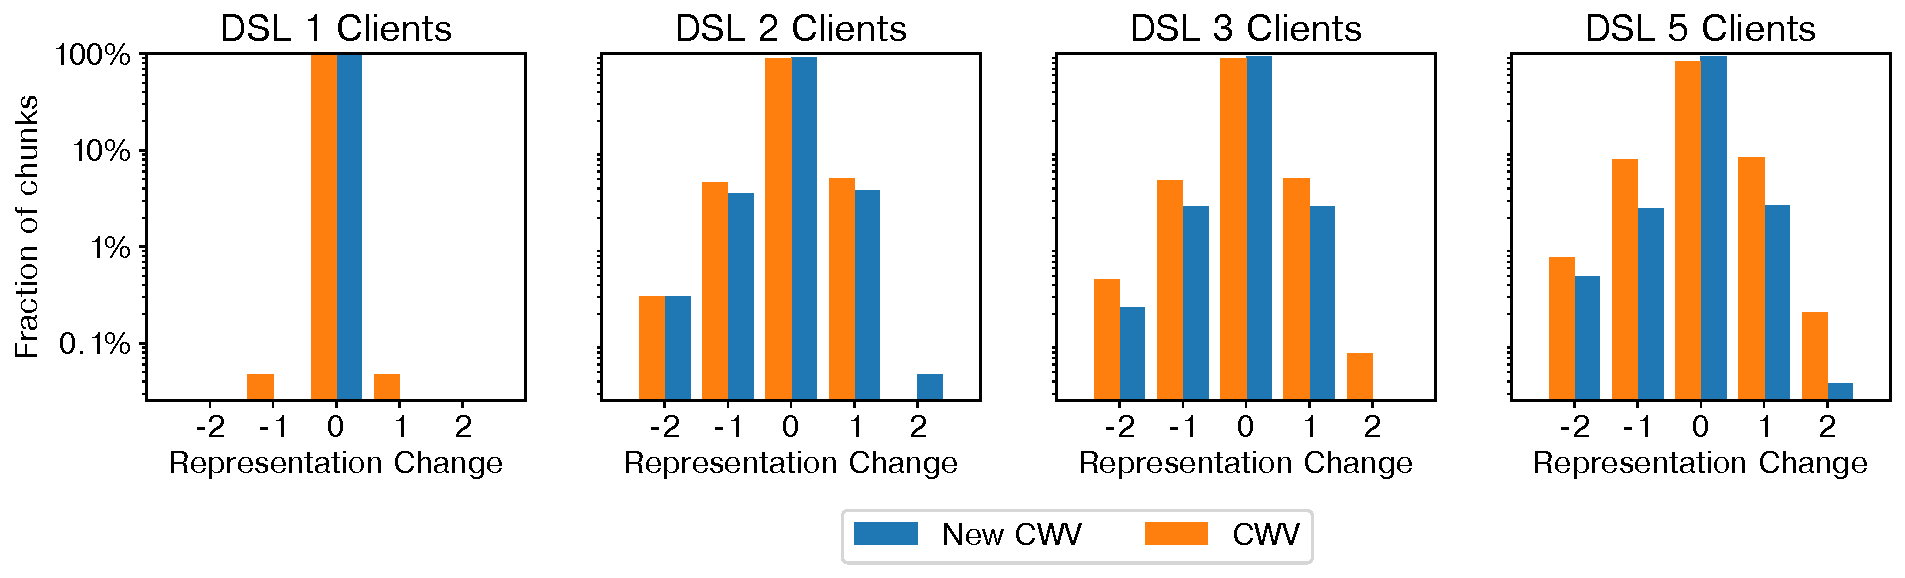
\includegraphics[width=\textwidth, keepaspectratio]{figures/bitrate_derivative_distribution.pdf}
  \caption{Absolute Bitrate Switches}
  \label{fig:bitrate-switches}
\end{figure*}

\begin{figure}
      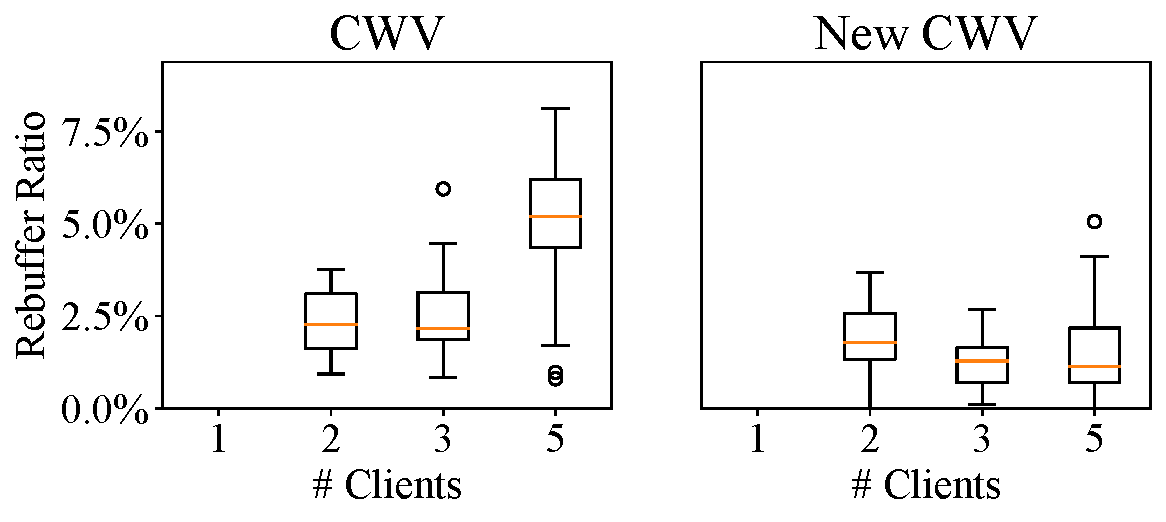
\includegraphics[width=.45\textwidth, keepaspectratio]{figures/Rebuffer_Ratio.pdf}
    \caption{Rebuffer Ratio}
    \label{fig:rebuffer-ratio}
\end{figure}



Next, we investigate whether the improved transport layer performance of New CWV translates into improved QoE at the application layer. To evaluate this, the rebuffer ratio and the bitrate switch frequency distribution and report results for the DSL case. 

% Figure \ref{fig:avg-oscillations} shows average bitrate oscillation. \todo{one/two sentences intuition about the scale}. Bitrate oscillation is typically lower when New CWV is enabled, and this is associated with improved QoE~\todo{\cite{..}}. This is a result of the higher, and less consistent, bandwidth estimates observed when New CWV is not enabled, as described in Section~\ref{sec:transport-impact}. These higher estimates lead to the client requesting chunks at a bitrate that the network cannot ultimately support, leading to increased oscillations and lower QoE. A similar pattern can be seen in Figure~\ref{fig:rebuffer-ratio}, which shows the rebuffer ratio.

Figure \ref{fig:bitrate-switches} shows the observed bitrate switch distribution. The figure shows that New CWV connections more persistently request the same bit-rate representation. The proportion of the requested chunks (y-axis) is shown using a logarithmic scale. The representation change (x-axis) is the magnitude of the bi-chunk bitrate switches. For example, a chunk played the same bit-rate as its preceding chunk, their difference is zero. If the current chunk is of the next higher encoding, compared to its predecessor, their difference is 1, and if it is of the next lower encoding the difference is -1, and so forth. We see that for the case with 5 clients, connections without New CWV experience non-zero quality switches for 17.4\% of the video duration, compared to 5.7\% for connections with New CWV. For a video consisting of just over 200 chunks, that 11.7\% difference means that on average New CWV connections see 24 fewer switches over the course of the video playback.

Figure \ref{fig:rebuffer-ratio} shows the percentage that the of the whole video playback that the connection spent in rebuffering state, i.e., no video play progress did not advance. Again, looking at the 5 client case, we see that New CWV not only achieves fewer switched, as already explained, but also experiences less rebuffering overall. The mean rebuffering values for the 5 client case are 1.5\% and 5\% for New CWV and CWV respectively. For a 10 minute video, that 3.5\% difference accounts for over 10 seconds of rebuffering time.

% For a 10 minute video, that 6\% difference accounts for 36 seconds shorter video rebuffering for New CWV connections throughout the video playback.

For brevity, we only report the DSL results, as in the FTTP cases our combination of clients and video encodings enabled all clients to stream at the highest quality without hitting the link limits. Similarly, this was the case for all FTTC simulations, except the 5 client one. In it, we observe similar patterns as those shown for DSL. For this reason, we believe that the problem we describe here would re-emerge for faster links as the network video demands increase as a factor of higher resolutions being widely deployed or as other network heavy applications start competing for the links' resources (e.g., Virtual Reality).

We conclude that New CWV achieves higher video stability when multiple clients are competing on a constrained link, with improved encoding stability and decreased rebuffering time. We have observed this behaviour mainly on the simulated DSL link, since our highest video encoding is just under 5Mbps, but in practice higher encodings are also used~\cite{online-youtube-encodings}.


%--------------------------------------------------------------------------------------------------
\subsection{Summary}
\label{sec:summary}

We have validated the throughput results observed by Nazir et al.~\cite{Nazir-2014-performance-evaluation-congestion-window-validation-dash-newcwv} (Figure~\ref{fig:throughput-clients}), but with observed higher packet loss where New CWV is not enabled (Figure~\ref{fig:transmission-after-idle}). Furthermore, our results demonstrate that New CWV's more consistent bandwidth measurements (Figure~\ref{fig:throughput-clients}) translate to fewer representation switches (Figure \ref{fig:bitrate-switches}). Finally, we also observed that the more consistent measurements better match the available network conditions, allowing clients using New CWV to better predict the network's capabilities and request chunks that can be delivered on time (Figure \ref{fig:rebuffer-ratio}).

%In Section \ref{sec:evaluation}, we saw that New CWV improves video stability by sacrificing some rendered picture quality for links with restrained capacities and multiple clients. We also, observed that when the there is sufficient link capacity to satisfy the most demanding representation, as expected the rendered quality is high and there are no stability issues. In other words, if the network resources are oversupplied with regard to the highest video requirement, there are no issues.  However, if the client is able to download at rate over the highest representation requirement, then whether the download happens 20\% or 50\% faster, makes no significant impact. The only real benefit is that the buffers at the client would fill quicker. Therefore, clients can potentially impose a maximum limit to their desired download rate and leave the rest of the link unused for other flows.
% ^ not sure what this adds: might just need rewording

%==================================================================================================
\section{Related Work}
\label{sec:related}

New CWV enhances the previous CWV algorithm~\cite{rfc2861-2000-padhye-congestion-window-validation}. Both CWV and New CWV attempt to solve the issue of connection resumption after an idle period in which TCP's view of the network has become stale. While CWV addresses the issue for bulk, network-limited applications, New CWV improves the algorithm for rate-limited applications. As a result of their changes, both algorithms alter TCP's send rate. This core idea, of altering TCP's sending dynamics, is not new. Building on work by Mathis et al.~\cite{Mathis-1997-the-macroscopic-behavior-tcp} and Padhye et al.~\cite{Padhye-1998-modelling-tcp-throughput}, there has been a significant volume of work on TCP friendliness and rate control~\cite{rfc-5348-tfrc,Rossi-2010-ledbat,Arun-2018-copa}, including for multimedia~\cite{Carlucci-2016-Analysis-WebRTC,Choi-2007-fairer-tfrc}.

While there has been much work at the transport layer, there has also been significant effort in attempting to reduce the impact of network and transport layer effects through rate adaption algorithms at the application layer. Three main concepts for adaptation algorithms have been proposed: throughput-based \cite{Sun-2016-cs2p, Jiang-2012-improving-fairness-http-video-festive}, buffer-based \cite{Spiteri-2016-BOLA,Huang-2015-A-buffer-based-approach-to-rate-adaptation-bba}, and hybrid \cite{Spiteri-2019-from-theory-to-practice-sabre,Wang-2016-squad}. Rate-based solutions~\cite{Li-2014-probe-and-adapt-panda,Liu-2011-rate-adaptation} have also been proposed, but these are not yet part of the DASH-IF reference implementation.

%As different adaptation algorithms were proposed, the need of metrics to evaluate and compare them arose. Early research provided metrics to evaluate the perceived QoE \cite{Cranley-2006-user-perception-adapting-video}. However, later \cite{Balachandran-2012-quest-for-internet-video-qoe} argued that no single combination of low-level metrics can provide a good QoE score for measuring video. Since then, QoE defining research relied on modelling and predictive patterns, however, a single agreed upon metric to measure to QoE has still not been found.

The work on general adaptation algorithms has slowed down with most recent proposals optimizing for specific cases (\cite{Karagkioules-2020-achieving-low-latency}). Partly, this is since latest general adaptation proposals had high complexity, without offering a substantial improvement \cite{Yin-2015-a-control-theoritic-approach} and ultimately did not make it to the mainline algorithms used in practice. In this work, we identified cases where the current state-of-the art algorithms fail to perform, e.g., multiple clients competing on a constrained link. Also, we showed that simple transport changes, such as the CWND sizing can have positive QoE impact in these cases with up to 4\% improved rebuffering and 12\% more stable chunk selection. With out work, we hope that we will open a discussion and allow more researchers to look into adapting the transport layer for video performance.

We believe that with changes to the transport layer, simple, network-reactive, throughput algorithms will be able to perform comparable to other more complex solutions, such as buffer-based algorithms. Thus, making simpler adaptation algorithms able to compete with the state-of-the-art complex ones. In turn, this could lead to a reduced overall complexity of the adaptation logic or enable different options for how adaptation algorithms could be improved.

%==================================================================================================
\section{Conclusions}
\label{sec:conclusion}

In this paper, we have shown that New CWV provides improved video playback stability. We compared video delivery with and without New CWV and validated the results shown by previous work \cite{Nazir-2014-performance-evaluation-congestion-window-validation-dash-newcwv}. We reported video delivery scenarios using emulated links representative for the commodity of last-mile links found in the UK and examined scenarios with different numbers of clients. We found that enabling New CWV for video connections can reduce the number of encoding switches throughout the connection by 12\% and can reduce the rebuffering time by up to 4\%.

Future work might look at the performance of these algorithms under more dynamic environments, for example if all clients join the session at random times or in the presence of other cross-traffic. 

%==================================================================================================
%\section{Acknowledgements}

% Acknowledge funding sources.

%==================================================================================================
% Set the bibliography style. Choose one of the following, depending on the
% document class being used:
%
%   \bibliographystyle{abbrv}                 When using article class
%   \bibliographystyle{IEEEtran}              When using IEEE style
%   \bibliographystyle{ACM-Reference-Format}  When using ACM style

\bibliographystyle{ACM-Reference-Format}

% Load the bibliography file(s) for this paper:
\bibliography{paper}

%==================================================================================================
% The following information gets written into the PDF file information:
\ifpdf
  \pdfinfo{
    /Title        (...)
    /Author       (...)
    /Subject      (...)
    /Keywords     (..., ..., ...)
    /CreationDate (D:20150827110616Z)
    /ModDate      (D:20150827110616Z)
    /Creator      (LaTeX)
    /Producer     (pdfTeX)
  }
  % Suppress unnecessary metadata, to ensure the PDF generated by pdflatex is
  % identical each time it is built. This needs pdfTeX 3.14159265-2.6-1.40.17
  % or later.
  \ifdefined\pdftrailerid
    \pdftrailerid{}
    \pdfsuppressptexinfo=15
  \fi
\fi


%==================================================================================================
\end{document}
% vim: set ts=2 sw=2 tw=75 et ai:
